\documentclass[12pt,]{article}
\usepackage{lmodern}
\usepackage{amssymb,amsmath}
\usepackage{ifxetex,ifluatex}
\usepackage{fixltx2e} % provides \textsubscript
\ifnum 0\ifxetex 1\fi\ifluatex 1\fi=0 % if pdftex
  \usepackage[T1]{fontenc}
  \usepackage[utf8]{inputenc}
\else % if luatex or xelatex
  \ifxetex
    \usepackage{mathspec}
  \else
    \usepackage{fontspec}
  \fi
  \defaultfontfeatures{Ligatures=TeX,Scale=MatchLowercase}
    \setmainfont[]{Times New Roman}
\fi
% use upquote if available, for straight quotes in verbatim environments
\IfFileExists{upquote.sty}{\usepackage{upquote}}{}
% use microtype if available
\IfFileExists{microtype.sty}{%
\usepackage{microtype}
\UseMicrotypeSet[protrusion]{basicmath} % disable protrusion for tt fonts
}{}
\usepackage[margin=2.54cm]{geometry}
\usepackage{hyperref}
\hypersetup{unicode=true,
            pdftitle={Linguistic Diversity in China and Influencing Environmental Factors},
            pdfauthor={Xin Wang},
            pdfborder={0 0 0},
            breaklinks=true}
\urlstyle{same}  % don't use monospace font for urls
\usepackage{color}
\usepackage{fancyvrb}
\newcommand{\VerbBar}{|}
\newcommand{\VERB}{\Verb[commandchars=\\\{\}]}
\DefineVerbatimEnvironment{Highlighting}{Verbatim}{commandchars=\\\{\}}
% Add ',fontsize=\small' for more characters per line
\usepackage{framed}
\definecolor{shadecolor}{RGB}{248,248,248}
\newenvironment{Shaded}{\begin{snugshade}}{\end{snugshade}}
\newcommand{\KeywordTok}[1]{\textcolor[rgb]{0.13,0.29,0.53}{\textbf{#1}}}
\newcommand{\DataTypeTok}[1]{\textcolor[rgb]{0.13,0.29,0.53}{#1}}
\newcommand{\DecValTok}[1]{\textcolor[rgb]{0.00,0.00,0.81}{#1}}
\newcommand{\BaseNTok}[1]{\textcolor[rgb]{0.00,0.00,0.81}{#1}}
\newcommand{\FloatTok}[1]{\textcolor[rgb]{0.00,0.00,0.81}{#1}}
\newcommand{\ConstantTok}[1]{\textcolor[rgb]{0.00,0.00,0.00}{#1}}
\newcommand{\CharTok}[1]{\textcolor[rgb]{0.31,0.60,0.02}{#1}}
\newcommand{\SpecialCharTok}[1]{\textcolor[rgb]{0.00,0.00,0.00}{#1}}
\newcommand{\StringTok}[1]{\textcolor[rgb]{0.31,0.60,0.02}{#1}}
\newcommand{\VerbatimStringTok}[1]{\textcolor[rgb]{0.31,0.60,0.02}{#1}}
\newcommand{\SpecialStringTok}[1]{\textcolor[rgb]{0.31,0.60,0.02}{#1}}
\newcommand{\ImportTok}[1]{#1}
\newcommand{\CommentTok}[1]{\textcolor[rgb]{0.56,0.35,0.01}{\textit{#1}}}
\newcommand{\DocumentationTok}[1]{\textcolor[rgb]{0.56,0.35,0.01}{\textbf{\textit{#1}}}}
\newcommand{\AnnotationTok}[1]{\textcolor[rgb]{0.56,0.35,0.01}{\textbf{\textit{#1}}}}
\newcommand{\CommentVarTok}[1]{\textcolor[rgb]{0.56,0.35,0.01}{\textbf{\textit{#1}}}}
\newcommand{\OtherTok}[1]{\textcolor[rgb]{0.56,0.35,0.01}{#1}}
\newcommand{\FunctionTok}[1]{\textcolor[rgb]{0.00,0.00,0.00}{#1}}
\newcommand{\VariableTok}[1]{\textcolor[rgb]{0.00,0.00,0.00}{#1}}
\newcommand{\ControlFlowTok}[1]{\textcolor[rgb]{0.13,0.29,0.53}{\textbf{#1}}}
\newcommand{\OperatorTok}[1]{\textcolor[rgb]{0.81,0.36,0.00}{\textbf{#1}}}
\newcommand{\BuiltInTok}[1]{#1}
\newcommand{\ExtensionTok}[1]{#1}
\newcommand{\PreprocessorTok}[1]{\textcolor[rgb]{0.56,0.35,0.01}{\textit{#1}}}
\newcommand{\AttributeTok}[1]{\textcolor[rgb]{0.77,0.63,0.00}{#1}}
\newcommand{\RegionMarkerTok}[1]{#1}
\newcommand{\InformationTok}[1]{\textcolor[rgb]{0.56,0.35,0.01}{\textbf{\textit{#1}}}}
\newcommand{\WarningTok}[1]{\textcolor[rgb]{0.56,0.35,0.01}{\textbf{\textit{#1}}}}
\newcommand{\AlertTok}[1]{\textcolor[rgb]{0.94,0.16,0.16}{#1}}
\newcommand{\ErrorTok}[1]{\textcolor[rgb]{0.64,0.00,0.00}{\textbf{#1}}}
\newcommand{\NormalTok}[1]{#1}
\usepackage{longtable,booktabs}
\usepackage{graphicx,grffile}
\makeatletter
\def\maxwidth{\ifdim\Gin@nat@width>\linewidth\linewidth\else\Gin@nat@width\fi}
\def\maxheight{\ifdim\Gin@nat@height>\textheight\textheight\else\Gin@nat@height\fi}
\makeatother
% Scale images if necessary, so that they will not overflow the page
% margins by default, and it is still possible to overwrite the defaults
% using explicit options in \includegraphics[width, height, ...]{}
\setkeys{Gin}{width=\maxwidth,height=\maxheight,keepaspectratio}
\IfFileExists{parskip.sty}{%
\usepackage{parskip}
}{% else
\setlength{\parindent}{0pt}
\setlength{\parskip}{6pt plus 2pt minus 1pt}
}
\setlength{\emergencystretch}{3em}  % prevent overfull lines
\providecommand{\tightlist}{%
  \setlength{\itemsep}{0pt}\setlength{\parskip}{0pt}}
\setcounter{secnumdepth}{5}
% Redefines (sub)paragraphs to behave more like sections
\ifx\paragraph\undefined\else
\let\oldparagraph\paragraph
\renewcommand{\paragraph}[1]{\oldparagraph{#1}\mbox{}}
\fi
\ifx\subparagraph\undefined\else
\let\oldsubparagraph\subparagraph
\renewcommand{\subparagraph}[1]{\oldsubparagraph{#1}\mbox{}}
\fi

%%% Use protect on footnotes to avoid problems with footnotes in titles
\let\rmarkdownfootnote\footnote%
\def\footnote{\protect\rmarkdownfootnote}

%%% Change title format to be more compact
\usepackage{titling}

% Create subtitle command for use in maketitle
\newcommand{\subtitle}[1]{
  \posttitle{
    \begin{center}\large#1\end{center}
    }
}

\setlength{\droptitle}{-2em}

  \title{Linguistic Diversity in China and Influencing Environmental Factors}
    \pretitle{\vspace{\droptitle}\centering\huge}
  \posttitle{\par}
  \subtitle{\url{https://github.com/nataliadxx/Environmental_Data_Analytics/tree/master/Final_Project}}
  \author{Xin Wang}
    \preauthor{\centering\large\emph}
  \postauthor{\par}
    \date{}
    \predate{}\postdate{}
  

\begin{document}
\maketitle
\begin{abstract}
This project aims to explore the pattern of linguistic diversity in
China and potential influence of environmental factors. With a dataset
derived from multiple sources, spatial visualization is realized, and
multiple linear regression models are built. The clear pattern is that
linguistic diversity is high Southwestern, Northwestern, Northeastern
China and Taiwan, which accords with regions that minor ethnic groups
inhabit. Yunnan Province produces the highest diversity. Results of
linear regression models show that the heterogeneity of topography is
the main environmental factor that facilitates the pattern of linguistic
diversity in China. Transportation efficiency, in contrast, may lead to
uniformity. Climatic variables have little influence on linguistic
diversity.
\end{abstract}

\newpage

\tableofcontents  \newpage
\listoffigures  \newpage

\section{Research Question and
Rationale}\label{research-question-and-rationale}

Languages are the production and reflection of human cultures. The
mechanisms of the formation of linguistic diversity or cultural
diversity have been discussed theoretically and empirically since 1990s.
Several explanations have been proposed by environmenal anthropologists
on the relationship between languages and the environment. The analysis
of this project is going to study whether environmental factors possibly
exert influence on language diversity in China, a country with over 50
nationalities, to testify some hypotheses.

Specifically, my research goals are: 1. Describe the spatial pattern of
linguistic diversity in China. 2. Test the influence of environmental
variables on linguistic diversity. The dataset includes information on
language richness distribution and environmental variables.

\newpage

\section{Dataset Information}\label{dataset-information}

Language richness data was collected from a linguistic monograph
``Languages in China'' (Sun et al. 2007). Climatic data was derived from
WorldClim (\url{http://www.worldclim.org/}). Topography indices were
calculated with SRTM digital elevation model (DEM)
(\url{http://datamirror.csdb.cn/}). Other environmental data came from
National Geomatics Center of China (\url{http://www.ngcc.cn/}).

The year of all variables is 2000. Variables are calculated in 50km*50km
grids.

Besides total richness of languages, the richness of each language
family and endemic languages are also listed here. Climatic indices
include mean annual temperature (MAT), minimum temperature of the
coldest month(mTCM), annual range of temperature (ART) and precipitation
seasonality (PSN). Among them, MAT and mTCM are indicators of overall
energy and productivity available, while ART and PSN represent the
climate variability. The zonal range of elevation inside each grid is
used as an index of topographical roughness. Other variables considered
are land cover types and river length, which is an indicator of
transportation efficiency.

The structure of the dataset is simplified as below.

\begin{longtable}[]{@{}llllll@{}}
\toprule
\begin{minipage}[b]{0.18\columnwidth}\raggedright\strut
Spatial coordinate\strut
\end{minipage} & \begin{minipage}[b]{0.08\columnwidth}\raggedright\strut
Climate\strut
\end{minipage} & \begin{minipage}[b]{0.11\columnwidth}\raggedright\strut
Topography\strut
\end{minipage} & \begin{minipage}[b]{0.17\columnwidth}\raggedright\strut
Language richness\strut
\end{minipage} & \begin{minipage}[b]{0.13\columnwidth}\raggedright\strut
River length\strut
\end{minipage} & \begin{minipage}[b]{0.16\columnwidth}\raggedright\strut
Habitat richness\strut
\end{minipage}\tabularnewline
\midrule
\endhead
\begin{minipage}[t]{0.18\columnwidth}\raggedright\strut
\strut
\end{minipage} & \begin{minipage}[t]{0.08\columnwidth}\raggedright\strut
\strut
\end{minipage} & \begin{minipage}[t]{0.11\columnwidth}\raggedright\strut
\strut
\end{minipage} & \begin{minipage}[t]{0.17\columnwidth}\raggedright\strut
\strut
\end{minipage} & \begin{minipage}[t]{0.13\columnwidth}\raggedright\strut
\strut
\end{minipage}\tabularnewline
\bottomrule
\end{longtable}

\newpage

\section{Exploratory Data Analysis and
Wrangling}\label{exploratory-data-analysis-and-wrangling}

\begin{Shaded}
\begin{Highlighting}[]
\NormalTok{dat <-}\StringTok{ }\KeywordTok{read.csv}\NormalTok{(}\StringTok{"China_language_data.csv"}\NormalTok{)}
\KeywordTok{colnames}\NormalTok{(dat)}
\end{Highlighting}
\end{Shaded}

\begin{verbatim}
##  [1] "lati"              "longi"             "MAT"              
##  [4] "mTCM"              "ART"               "PSN"              
##  [7] "TOPO"              "DEMSTD"            "languages"        
## [10] "endemic.languages" "Sino.Tibetan"      "Altaic"           
## [13] "Austronesian"      "Austroasiatic"     "PD"               
## [16] "NRI"               "river123"          "river4"           
## [19] "river5"            "river_all"         "broad.leave"      
## [22] "shrub"             "grassland"         "agricultural"     
## [25] "coniferous"        "forest"            "veg_rich"         
## [28] "veg_SN"
\end{verbatim}

\begin{Shaded}
\begin{Highlighting}[]
\KeywordTok{dim}\NormalTok{(dat)}
\end{Highlighting}
\end{Shaded}

\begin{verbatim}
## [1] 3688   28
\end{verbatim}

\begin{Shaded}
\begin{Highlighting}[]
\KeywordTok{head}\NormalTok{(dat)}
\end{Highlighting}
\end{Shaded}

\begin{verbatim}
##      lati   longi      MAT     mTCM      ART      PSN TOPO  DEMSTD
## 1 18.3753 109.340 24.38897 15.55873 15.37884 81.98048 1034 201.350
## 2 18.3509 109.780 25.22693 16.57471 15.12147 80.37083  644 122.918
## 3 18.8185 108.922 23.64081 14.03507 16.84104 81.34961 1604 271.717
## 4 18.7962 109.365 22.74407 13.27876 16.57161 79.99481 1307 272.335
## 5 18.7716 109.807 23.31010 14.03340 16.34060 76.97474 1705 304.039
## 6 18.7446 110.249 24.62666 15.47077 16.36894 72.26311 1004 162.361
##   languages endemic.languages Sino.Tibetan Altaic Austronesian
## 1         4                 2            3      0            1
## 2         4                 2            3      0            1
## 3         5                 3            5      0            0
## 4         5                 3            4      0            1
## 5         3                 1            3      0            0
## 6         3                 1            3      0            0
##   Austroasiatic PD      NRI river123 river4  river5 river_all broad.leave
## 1             0 13 1.474811        0      0  0.0000    0.0000    168.0420
## 2             0 13 1.474811        0      0  0.0000    0.0000    579.7556
## 3             0 10 3.932410        0      0 46.8139   46.8139   1254.0772
## 4             0 14 2.260451        0      0 86.6415   86.6415   1429.9099
## 5             0  8 2.006558        0      0  0.0000    0.0000   1928.3290
## 6             0  8 2.006558        0      0  0.0000    0.0000   1311.1682
##       shrub grassland agricultural coniferous    forest veg_rich    veg_SN
## 1 1097.3900         0     530.8145          0  168.0420        3 0.8871714
## 2  688.6900         0     125.3720          0  579.7556        3 0.9393403
## 3  578.7535         0     652.4390          0 1254.0772        3 1.0436586
## 4  473.0450         0     597.0450          0 1429.9099        3 0.9868879
## 5  571.6710         0       0.0000          0 1928.3290        2 0.5509916
## 6  384.3394         0     259.7964          0 1311.1682        3 0.8740687
\end{verbatim}

\begin{Shaded}
\begin{Highlighting}[]
\KeywordTok{summary}\NormalTok{(dat}\OperatorTok{$}\NormalTok{languages)}
\end{Highlighting}
\end{Shaded}

\begin{verbatim}
##    Min. 1st Qu.  Median    Mean 3rd Qu.    Max. 
##   1.000   1.000   2.000   2.836   3.000  16.000
\end{verbatim}

\begin{Shaded}
\begin{Highlighting}[]
\KeywordTok{summary}\NormalTok{(dat}\OperatorTok{$}\NormalTok{Sino.Tibetan)}
\end{Highlighting}
\end{Shaded}

\begin{verbatim}
##    Min. 1st Qu.  Median    Mean 3rd Qu.    Max. 
##   1.000   1.000   1.000   1.977   2.000  15.000
\end{verbatim}

\begin{Shaded}
\begin{Highlighting}[]
\KeywordTok{summary}\NormalTok{(dat}\OperatorTok{$}\NormalTok{Altaic)}
\end{Highlighting}
\end{Shaded}

\begin{verbatim}
##    Min. 1st Qu.  Median    Mean 3rd Qu.    Max. 
##  0.0000  0.0000  0.0000  0.6185  1.0000  9.0000
\end{verbatim}

\begin{Shaded}
\begin{Highlighting}[]
\KeywordTok{summary}\NormalTok{(dat}\OperatorTok{$}\NormalTok{Austronesian)}
\end{Highlighting}
\end{Shaded}

\begin{verbatim}
##     Min.  1st Qu.   Median     Mean  3rd Qu.     Max. 
##  0.00000  0.00000  0.00000  0.02386  0.00000 12.00000
\end{verbatim}

\begin{Shaded}
\begin{Highlighting}[]
\KeywordTok{summary}\NormalTok{(dat}\OperatorTok{$}\NormalTok{Austroasiatic)}
\end{Highlighting}
\end{Shaded}

\begin{verbatim}
##    Min. 1st Qu.  Median    Mean 3rd Qu.    Max. 
## 0.00000 0.00000 0.00000 0.03308 0.00000 5.00000
\end{verbatim}

\begin{Shaded}
\begin{Highlighting}[]
\KeywordTok{shapiro.test}\NormalTok{(dat}\OperatorTok{$}\NormalTok{MAT)}
\end{Highlighting}
\end{Shaded}

\begin{verbatim}
## 
##  Shapiro-Wilk normality test
## 
## data:  dat$MAT
## W = 0.96955, p-value < 2.2e-16
\end{verbatim}

\begin{Shaded}
\begin{Highlighting}[]
\KeywordTok{shapiro.test}\NormalTok{(dat}\OperatorTok{$}\NormalTok{mTCM)}
\end{Highlighting}
\end{Shaded}

\begin{verbatim}
## 
##  Shapiro-Wilk normality test
## 
## data:  dat$mTCM
## W = 0.94577, p-value < 2.2e-16
\end{verbatim}

\begin{Shaded}
\begin{Highlighting}[]
\KeywordTok{shapiro.test}\NormalTok{(dat}\OperatorTok{$}\NormalTok{TOPO)}
\end{Highlighting}
\end{Shaded}

\begin{verbatim}
## 
##  Shapiro-Wilk normality test
## 
## data:  dat$TOPO
## W = 0.91412, p-value < 2.2e-16
\end{verbatim}

\begin{figure}
\centering
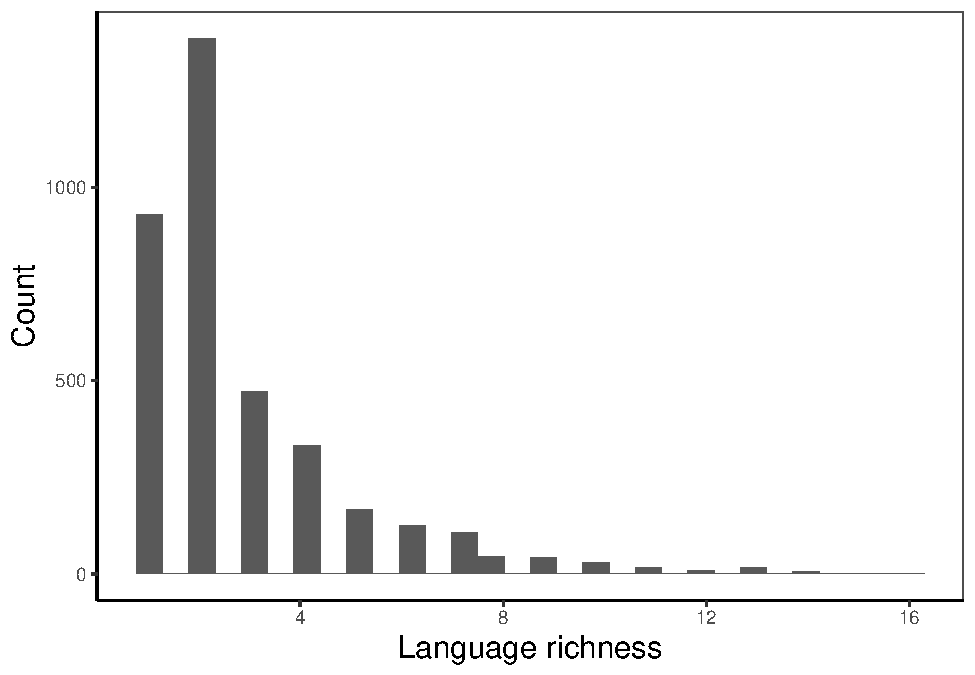
\includegraphics{Project_Template_files/figure-latex/unnamed-chunk-2-1.pdf}
\caption{Distribution of language richness in each grid}
\end{figure}

\begin{figure}
\centering
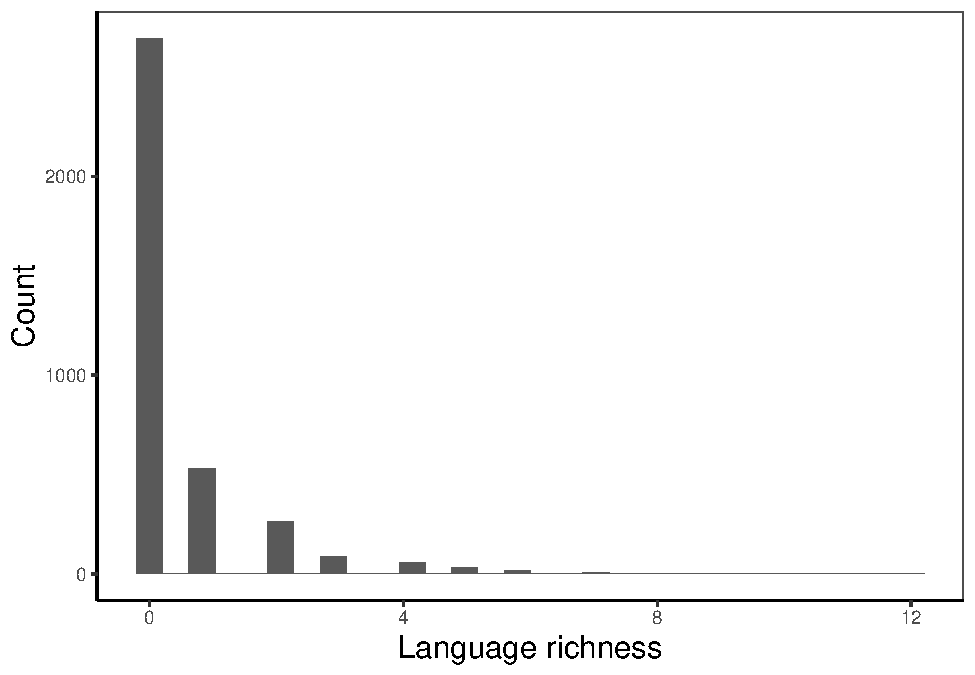
\includegraphics{Project_Template_files/figure-latex/unnamed-chunk-3-1.pdf}
\caption{Distribution of endemic language richness in each grid}
\end{figure}

\begin{figure}
\centering
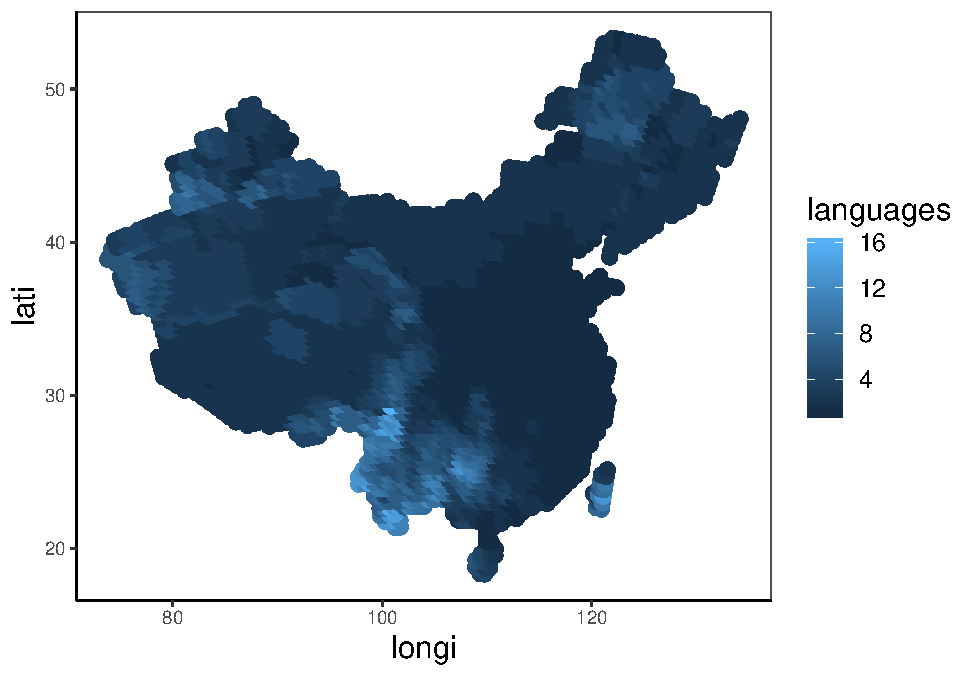
\includegraphics{Project_Template_files/figure-latex/unnamed-chunk-4-1.pdf}
\caption{Spatial range of the data}
\end{figure}

The goal of previous exploration steps is to get a sketchy idea of the
data. There are totally 3688 grids in the dataset. There are less than 4
languages in most area, but where languages are most diverse, there can
be up to 16 languages in a 50km??50km range. In terms of language
families, Sino-Tibetan and Altaic languages seem to be far more than
Austronesian and Austroasiatic. Most grids do not have endemic language
within it, but the most diverse one possesses 12 endemic languages. The
location of the points is shown on a map.

\newpage

\section{Analysis}\label{analysis}

\begin{Shaded}
\begin{Highlighting}[]
\NormalTok{model1 <-}\StringTok{ }\KeywordTok{lm}\NormalTok{(}\DataTypeTok{data =}\NormalTok{ dat, languages }\OperatorTok{~}\StringTok{ }\NormalTok{MAT}\OperatorTok{+}\NormalTok{mTCM)}
\KeywordTok{summary}\NormalTok{(model1)}
\end{Highlighting}
\end{Shaded}

\begin{verbatim}
## 
## Call:
## lm(formula = languages ~ MAT + mTCM, data = dat)
## 
## Residuals:
##     Min      1Q  Median      3Q     Max 
## -2.5944 -1.4205 -0.4321  0.7842 12.8665 
## 
## Coefficients:
##              Estimate Std. Error t value Pr(>|t|)    
## (Intercept)  4.983457   0.187412   26.59   <2e-16 ***
## MAT         -0.120582   0.011458  -10.52   <2e-16 ***
## mTCM         0.097579   0.008038   12.14   <2e-16 ***
## ---
## Signif. codes:  0 '***' 0.001 '**' 0.01 '*' 0.05 '.' 0.1 ' ' 1
## 
## Residual standard error: 2.143 on 3685 degrees of freedom
## Multiple R-squared:  0.0393, Adjusted R-squared:  0.03878 
## F-statistic: 75.37 on 2 and 3685 DF,  p-value: < 2.2e-16
\end{verbatim}

\begin{Shaded}
\begin{Highlighting}[]
\NormalTok{model2 <-}\StringTok{ }\KeywordTok{lm}\NormalTok{(}\DataTypeTok{data =}\NormalTok{ dat, languages }\OperatorTok{~}\StringTok{ }\NormalTok{ART}\OperatorTok{+}\NormalTok{PSN)}
\KeywordTok{summary}\NormalTok{(model2)}
\end{Highlighting}
\end{Shaded}

\begin{verbatim}
## 
## Call:
## lm(formula = languages ~ ART + PSN, data = dat)
## 
## Residuals:
##     Min      1Q  Median      3Q     Max 
## -2.8829 -1.4643 -0.4346  0.7355 12.5821 
## 
## Coefficients:
##              Estimate Std. Error t value Pr(>|t|)    
## (Intercept)  4.599640   0.171284  26.854  < 2e-16 ***
## ART         -0.059635   0.003864 -15.432  < 2e-16 ***
## PSN          0.006035   0.001657   3.643 0.000273 ***
## ---
## Signif. codes:  0 '***' 0.001 '**' 0.01 '*' 0.05 '.' 0.1 ' ' 1
## 
## Residual standard error: 2.118 on 3685 degrees of freedom
## Multiple R-squared:  0.06161,    Adjusted R-squared:  0.06111 
## F-statistic:   121 on 2 and 3685 DF,  p-value: < 2.2e-16
\end{verbatim}

\begin{Shaded}
\begin{Highlighting}[]
\NormalTok{model3 <-}\StringTok{ }\KeywordTok{lm}\NormalTok{(}\DataTypeTok{data =}\NormalTok{ dat, languages }\OperatorTok{~}\StringTok{ }\NormalTok{TOPO}\OperatorTok{+}\NormalTok{veg_rich)}
\KeywordTok{summary}\NormalTok{(model3)}
\end{Highlighting}
\end{Shaded}

\begin{verbatim}
## 
## Call:
## lm(formula = languages ~ TOPO + veg_rich, data = dat)
## 
## Residuals:
##    Min     1Q Median     3Q    Max 
## -5.527 -1.247 -0.462  0.659 11.857 
## 
## Coefficients:
##              Estimate Std. Error t value Pr(>|t|)    
## (Intercept) 1.589e+00  8.020e-02  19.813   <2e-16 ***
## TOPO        9.044e-04  3.644e-05  24.815   <2e-16 ***
## veg_rich    6.944e-02  2.888e-02   2.404   0.0163 *  
## ---
## Signif. codes:  0 '***' 0.001 '**' 0.01 '*' 0.05 '.' 0.1 ' ' 1
## 
## Residual standard error: 2.011 on 3685 degrees of freedom
## Multiple R-squared:  0.1541, Adjusted R-squared:  0.1536 
## F-statistic: 335.6 on 2 and 3685 DF,  p-value: < 2.2e-16
\end{verbatim}

\begin{Shaded}
\begin{Highlighting}[]
\NormalTok{model4 <-}\StringTok{ }\KeywordTok{lm}\NormalTok{(}\DataTypeTok{data =}\NormalTok{ dat, languages }\OperatorTok{~}\StringTok{ }\NormalTok{river_all)}
\KeywordTok{summary}\NormalTok{(model4)}
\end{Highlighting}
\end{Shaded}

\begin{verbatim}
## 
## Call:
## lm(formula = languages ~ river_all, data = dat)
## 
## Residuals:
##     Min      1Q  Median      3Q     Max 
## -2.1183 -1.1183 -0.8534  0.4688 13.2517 
## 
## Coefficients:
##               Estimate Std. Error t value Pr(>|t|)    
## (Intercept)  3.1182862  0.0530168   58.82  < 2e-16 ***
## river_all   -0.0031694  0.0004396   -7.21 6.76e-13 ***
## ---
## Signif. codes:  0 '***' 0.001 '**' 0.01 '*' 0.05 '.' 0.1 ' ' 1
## 
## Residual standard error: 2.17 on 3686 degrees of freedom
## Multiple R-squared:  0.01391,    Adjusted R-squared:  0.01364 
## F-statistic: 51.98 on 1 and 3686 DF,  p-value: 6.757e-13
\end{verbatim}

\begin{figure}
\centering
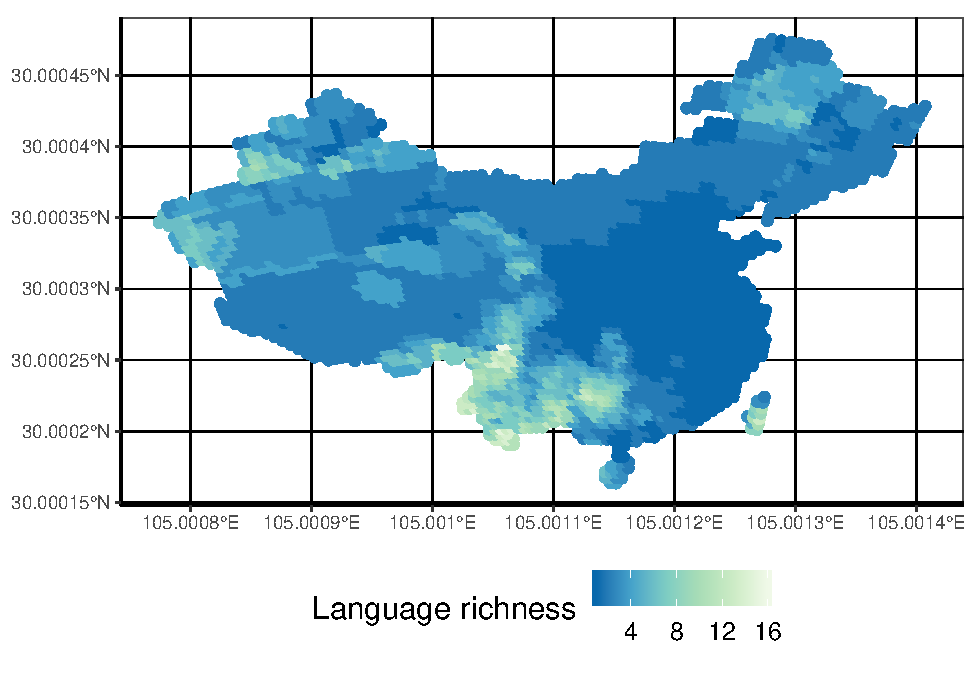
\includegraphics{Project_Template_files/figure-latex/unnamed-chunk-6-1.pdf}
\caption{Spatial distribution of linguistic diversity in China}
\end{figure}

\begin{figure}
\centering
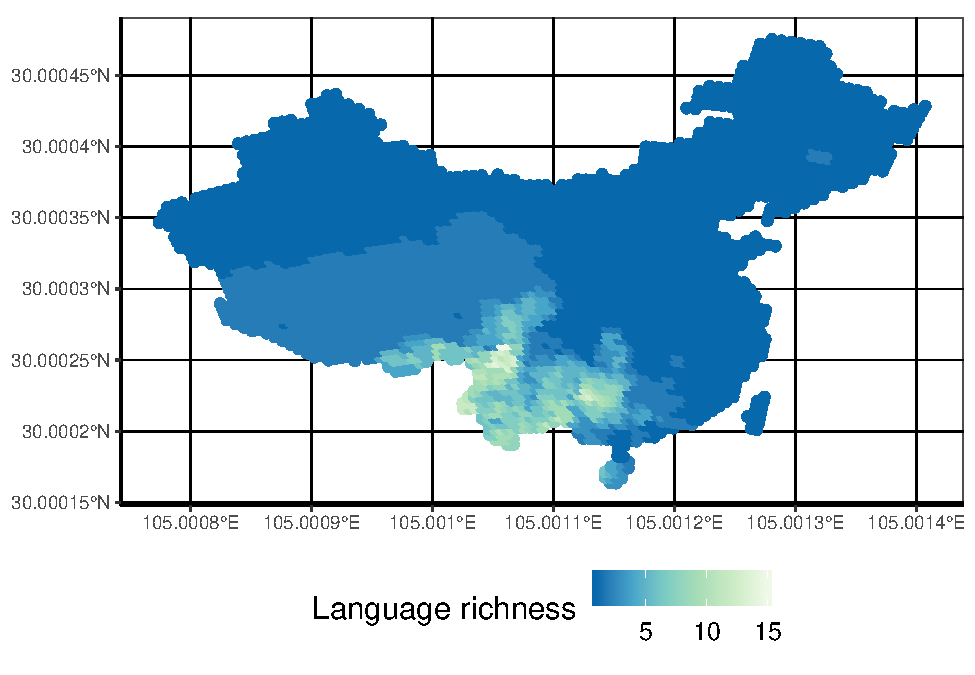
\includegraphics{Project_Template_files/figure-latex/unnamed-chunk-7-1.pdf}
\caption{Spatial distribution of Sino-Tibetan languages}
\end{figure}

\begin{figure}
\centering
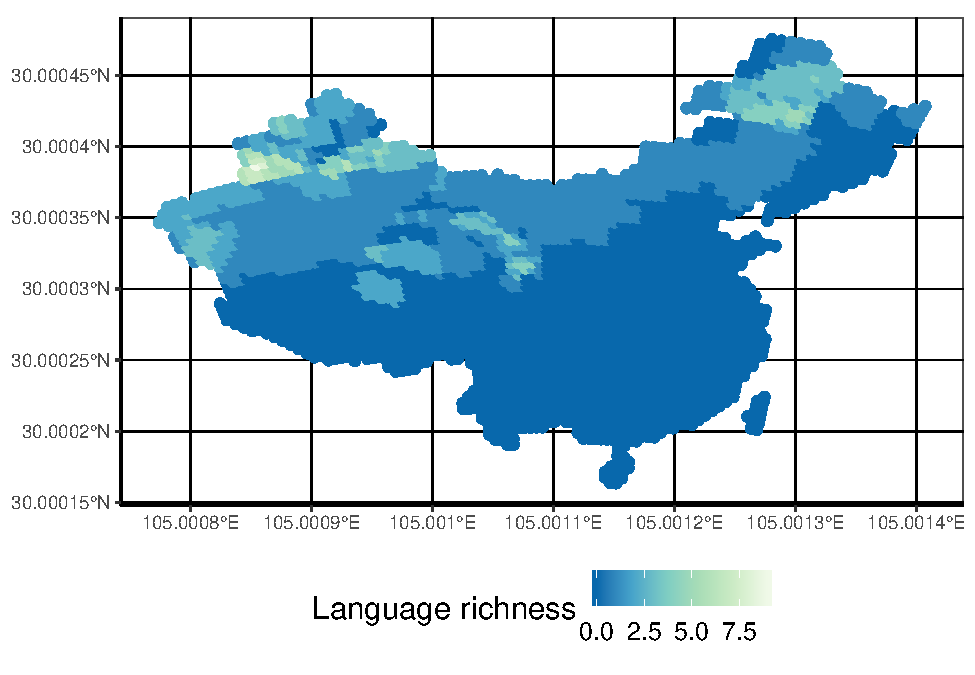
\includegraphics{Project_Template_files/figure-latex/unnamed-chunk-8-1.pdf}
\caption{Spatial distribution of Altaic languages}
\end{figure}

\begin{figure}
\centering
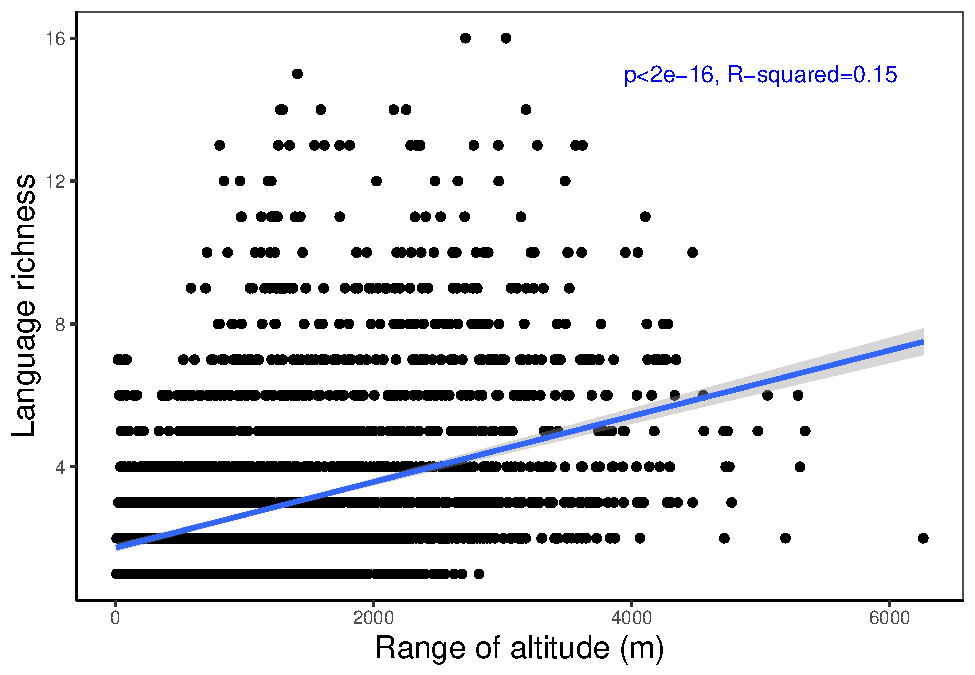
\includegraphics{Project_Template_files/figure-latex/unnamed-chunk-9-1.pdf}
\caption{Language richness to topographic roughness}
\end{figure}

Shapiro-Wilk normality tests in previous steps indicate that many
environmental variables do not approximate normal distributions.
However, since the dataset is large (over 3k observations), linear
regression will still be adopted.

In this case, environmental variables and language richness, the
responsive variable, are all continuos. Therefore, 4 multiple and single
linear regression models are used to test the following hypotheses. 1.
Areas with high energy and productivity develop more languages, which is
analogous to biodiversity. MAT and mTCM are explanatory variables. 2.
Areas with high climatic variability tend to have less languages because
communities may ally to resist variability. ART and PSN are explanatory
variables. 3. High habitat heterogeneity tend to develop more languages.
Topograhic roughness and habitat richness are explanatory variables. 4.
Areas with efficient transportation are likely to have less languages as
there is more frequent communication between communities. River length
is the explanatory variable.

\newpage

\section{Summary and Conclusions}\label{summary-and-conclusions}

 From the maps, the spatial pattern of linguistic diversity is
perceivable. Overall, linguistic diversity is low in southeastern,
central and northern China, while in southwestern, northwestern,
northeastern China and Taiwan, the diversity appears relatively high.
Yunnan Province, in the very southwestern corner, produces the highest
diversity. Specifically, the hotspot of Sino-Tibetan languages is the
southwestern part, while Altaic languages are mostly distributed in
northern part of the country.

From the results of linear regression models, the 4 hypotheses are
tested. Hypothesis 1 does not work here as the coefficient of MAT is
negative. Similarly, hypothesis 2 is rejected as the coefficient of ART
is negative. Therefore, climate may not be a determinant factor of
language formation in China. Hypothesis 3 is proved here, although the
effect of habitat richness is not as significant as that of topographic
roughness. This is parallel with the reality in Yunnan, where mountains
and river valleys are arranged in lines. Finally, although the
indicator, river length, is admittedly too simple to represent
transportation condition, hypothesis 4 is accepted.

To conclude, the heterogeneity of topography is the main environmental
factor that facilitates the pattern of linguistic diversity in China.
Transportation efficiency, in contrast, may lead to uniformity. Climatic
variables have little influence on linguistic diversity.


\end{document}
